\section{Arithmetic task}

The aim of the ``Arithmetic task'' is to directly test arithmetic models ability to extrapolate beyond the training range. Additionally, our generalized version provides a high degree of flexibility in how the input is shaped, sampled, and the problem complexity.

Our ``arithmetic task'' is identical to the ``simple function task'' in the NALU paper \cite{trask-nalu}. However, as they do not describe their setup in details, we use the setup from \citet{maep-madsen-johansen-2019}, which provide Algorithm \ref{tab:simple-function-task-defaults}, an evaluation-criterion to if and when the model has converged, the sparsity error, as well as methods for computing confidence intervals for success-rate and the sparsity error.

\begin{figure}[h]
\centering
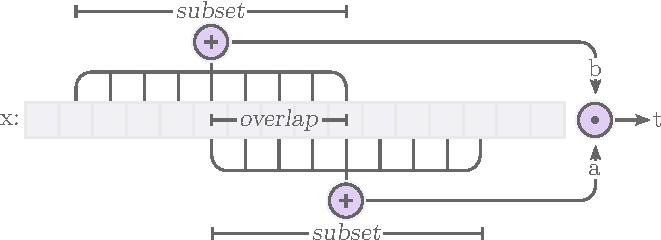
\includegraphics[scale=0.7]{graphics/function_task_static_problem.pdf}
\caption{Shows how the dataset is parameterized.}
\label{fig:simple-function-task-problem}
\end{figure}

\subsection{Dataset generation}
\label{sec:appendix:simple-function-task:data-generation}

The goal is to sum two random subsets of a vector $\mathbf{x}$ ($a$ and $b$), and perform an arithmetic operation on these ($a \circ b$).

\begin{equation}
    a = \sum_{i=s_{1,\mathrm{start}}}^{s_{1,\mathrm{end}}} x_i, \quad b = \sum_{i=s_{2,\mathrm{start}}}^{s_{2,\mathrm{end}}} x_i, \quad t = a \circ b
\end{equation}

Algorithm \ref{alg:simple-function-task-generator} defines the exact procedure to generate the data, where an interpolation range will be used for training and validation and an extrapolation range will be used for testing. Default values are defined in table \ref{tab:simple-function-task-defaults}.

\begin{table}[h]
\caption{Default dataset parameters for ``Arithmetic task''}
\label{tab:simple-function-task-defaults}
\centering
\begin{tabular}{cc}
\begin{minipage}{.4\linewidth}
\begin{tabular}{r l}
\toprule
 Parameter name & Default value \\
 \midrule
 Input size & 100 \\
 Subset ratio & 0.25 \\
 Overlap ratio & 0.5 \\
 \bottomrule
\end{tabular}
\end{minipage} &
\begin{minipage}{.4\linewidth}
\begin{tabular}{r l}
\toprule
 Parameter name & Default value \\
 \midrule
 Interpolation range & $U[1,2]$ \\
 Extrapolation range & $U[2,6]$ \\
 \\
 \bottomrule
\end{tabular}
\end{minipage}
\end{tabular}
\end{table}

\begin{algorithm}[h]
  \caption{Dataset generation algorithm for ``Arithmetic task''}
  \begin{algorithmic}[1]
    \Function{Dataset}{${\Call{Op}{\cdot, \cdot}: \mathrm{Operation}}$, ${i: \mathrm{Input Size}}$, ${s: \mathrm{Subset Ratio}}$, ${o: \mathrm{Overlap Ratio}}$, ${\hspace{3cm}R: \mathrm{Range}}$}
      \Let{$\mathbf{x}$}{\Call{Uniform}{$R_{lower}, R_{upper}, i$}} \Comment{Sample $i$ elements uniformly}
      \Let{$k$}{\Call{Uniform}{$0, 1 - 2s - o$}} \Comment{Sample offset}
      \Let{$a$}{\Call{Sum}{$\mathbf{x}[ik:i(k+s)]$}} \Comment{Create sum $a$ from subset}
      \Let{$b$}{\Call{Sum}{$\mathbf{x}[i(k+s-o):i (k+2s-0)]$}} \Comment{Create sum $b$ from subset}
      \Let{$t$}{\Call{Op}{$a, b$}} \Comment{Perform operation on $a$ and $b$}
      \State \Return{$x, t$}
    \EndFunction
  \end{algorithmic}
  \label{alg:simple-function-task-generator}
\end{algorithm}

\subsection{Model defintions and setup}

Models are defined in table \ref{tab:simple-function-task-model-defintions} and are all optimized with Adam optimization \cite{adam-optimization} using default parameters, and trained over $5 \cdot 10^6$ iterations. Training takes about 8 hours on a single CPU core(\text{8-Core Intel Xeon E5-2665 2.4GHz}). We run 19150 experiments on a HPC cluster.

The training dataset is continuously sampled from the interpolation range where a different seed is used for each experiment, all experiments use a mini-batch size of 128 observations, a fixed validation dataset with $1 \cdot 10^4$ observations sampled from the interpolation range, and a fixed test dataset with $1 \cdot 10^4$ observations sampled from the extrapolation range.

\begin{table}[h]
\caption{Model definitions}
\label{tab:simple-function-task-model-defintions}
\centering
\begin{tabular}{r l l l l l}
\toprule
 Model & Layer 1 & Layer 2 & $\hat{\lambda}_{\mathrm{sparse}}$ & $\lambda_{\mathrm{start}}$ & $\lambda_{\mathrm{end}}$ \\
 \midrule
 NMU & NAU & NMU & 10 & $10^6$ & $2 \cdot 10^6$ \\
 NAU & NAU & NAU & 0.01 & $5 \cdot 10^3$ & $5 \cdot 10^4$ \\
 $\mathrm{NAC}_{\bullet}$ & $\mathrm{NAC}_{+}$ & $\mathrm{NAC}_{\bullet}$ & -- & -- & -- \\
 $\mathrm{NAC}_{\bullet,\sigma}$ & $\mathrm{NAC}_{+}$ & $\mathrm{NAC}_{\bullet,\sigma}$ & -- & -- & -- \\
 $\mathrm{NAC}_{\bullet,\mathrm{NMU}}$ & $\mathrm{NAC}_{+}$ & $\mathrm{NAC}_{\bullet,\mathrm{NMU}}$ & 10 & $10^6$ & $2 \cdot 10^6$ \\
 $\mathrm{NAC}_{+}$ & $\mathrm{NAC}_{+}$ & $\mathrm{NAC}_{+}$ & -- & -- & -- \\
 NALU & NALU & NALU & -- & -- & -- \\
 Linear & Linear & Linear & -- & -- & -- \\
 ReLU & ReLU & ReLU & -- & -- & -- \\
 ReLU6 & ReLU6 & ReLU6 & -- & -- & -- \\
 \bottomrule
\end{tabular}
\end{table}

\subsection{Ablation study}
\label{sec:appendix:ablation-study}
To validate our model, we perform an ablation on the multiplication problem. Some noteworthy observations:

\begin{enumerate}
    \item None of the $W$ constraints, such as $\mathcal{R}_{sparse}$ and clamping W to be in $[0, 1]$, are necessary when the hidden size is just $2$.
    \item Removing the $\mathcal{R}_{sparse}$ causes the NMU to immediately fail for larger hidden sizes.
    \item Removing the clamping of W does not cause much difference. This is because $\mathcal{R}_{sparse}$ also constrains $W$ outside of $[0, 1]$. The regularizer used here is $\mathcal{R}_{sparse} = \min(|W|, |1 - W|)$, which is identical to the one used in other experiments in $[0, 1]$, but is also valid outside $[0, 1]$. Doing this gives only a slightly slower convergence. Although, this can not be guaranteed in general, as the regularizer is omitted during the initial optimization.
    \item Removing both constraints, gives a somewhat satisfying solution, but with a lower success-rate, slower convergence, and higher sparsity error.
\end{enumerate}

In conclusion both constraints are valuable, as they provide faster convergence and a sparser solution, but they are not critical to the success-rate of the NMU.

\begin{figure}[h]
\centering
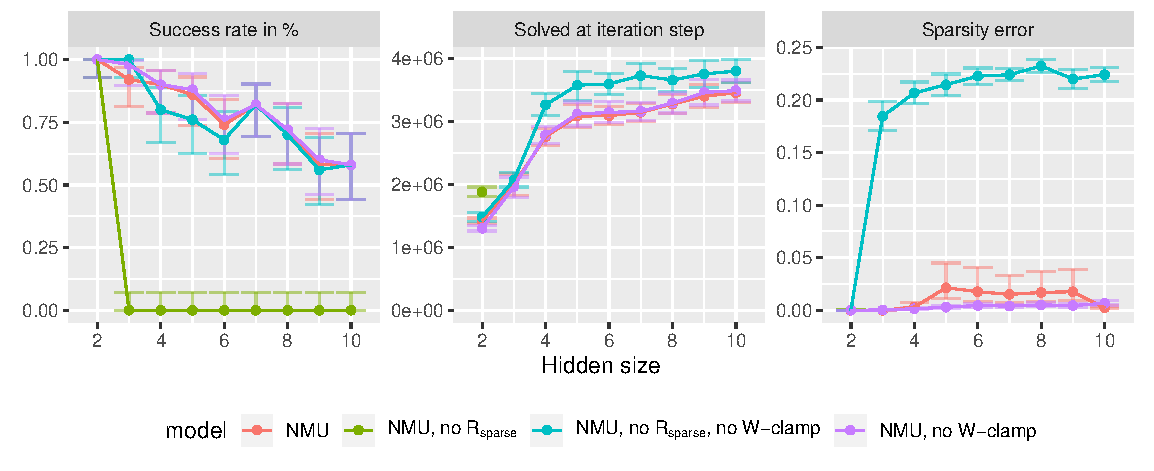
\includegraphics[width=\linewidth]{results/simple_function_static_mul_hidden_size_ablation.pdf}
\caption{Ablation study where $\mathcal{R}_{sparse}$ is removed and the clamping of W is removed. There are 50 experiments with different seeds, for each configuration.}
\label{fig:simple-function-static-ablation}
\end{figure}

\subsection{Effect of dataset parameter}
\label{sec:appendix-simple-function-task:dataset-parameter-effect}

To stress test the models on the multiplication task, we vary the dataset parameters one at a time while keeping the others at their default value (default values in table \ref{tab:simple-function-task-defaults}). Each runs for 50 experiments with different seeds. The results, are visualized in figure \ref{fig:simple-function-static-dataset-parameters-boundary}.

In figure \ref{fig:simple-function-static-theoreical-claims-experiment}, the interpolation-range is changed, therefore the extrapolation-range needs to be changed such it doesn't overlap. For each interpolation-range the following extrapolation-range is used: ${\mathrm{U}[-2,-1] \text{ uses } \mathrm{U}[-6,-2]}$, ${\mathrm{U}[-2,2] \text{ uses } \mathrm{U}[-6,-2] \cup \mathrm{U}[2,6]}$, ${\mathrm{U}[0,1] \text{ uses } \mathrm{U}[1,5]}$, ${\mathrm{U}[0.1,0.2] \text{ uses } \mathrm{U}[0.2,2]}$, ${\mathrm{U}[1.1,1.2] \text{ uses } \mathrm{U}[1.2,6]}$, ${\mathrm{U}[1,2] \text{ uses } \mathrm{U}[2,6]}$, ${\mathrm{U}[10, 20] \text{ uses } \mathrm{U}[20, 40]}$.

\begin{figure}[h]
\centering
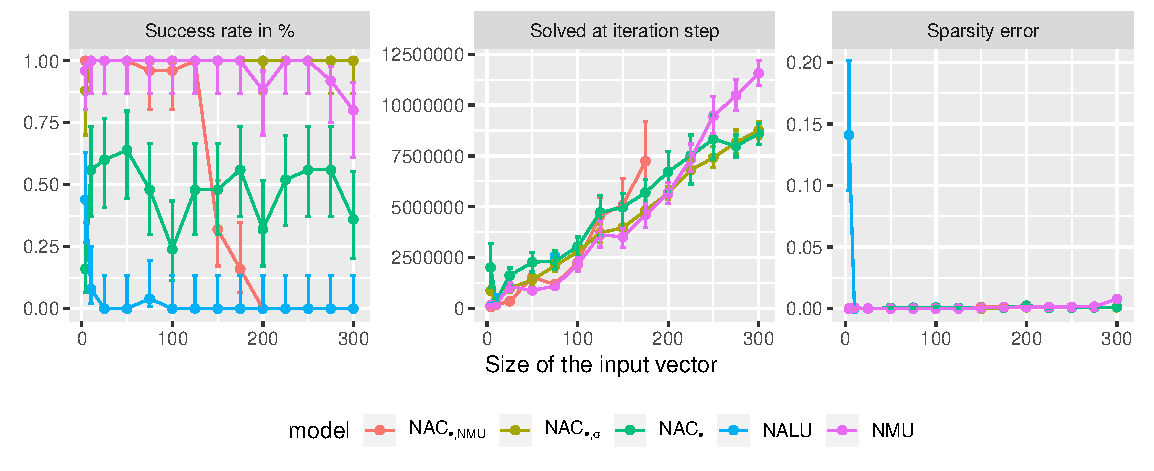
\includegraphics[width=\linewidth,trim={0 1.3cm 0 0},clip]{results/simple_function_static_mul_input_size.pdf}
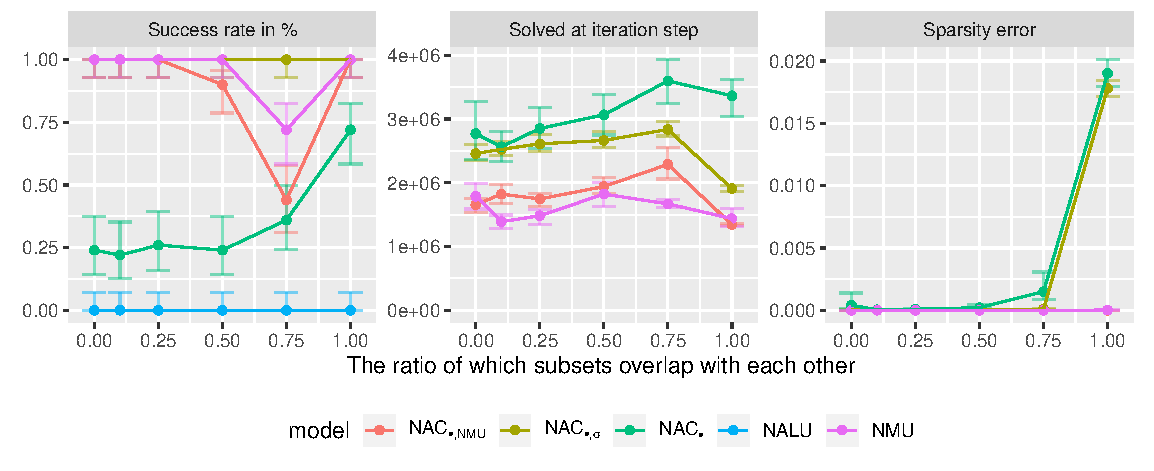
\includegraphics[width=\linewidth,trim={0 1.3cm 0 0.809cm},clip]{results/simple_function_static_mul_overlap.pdf}
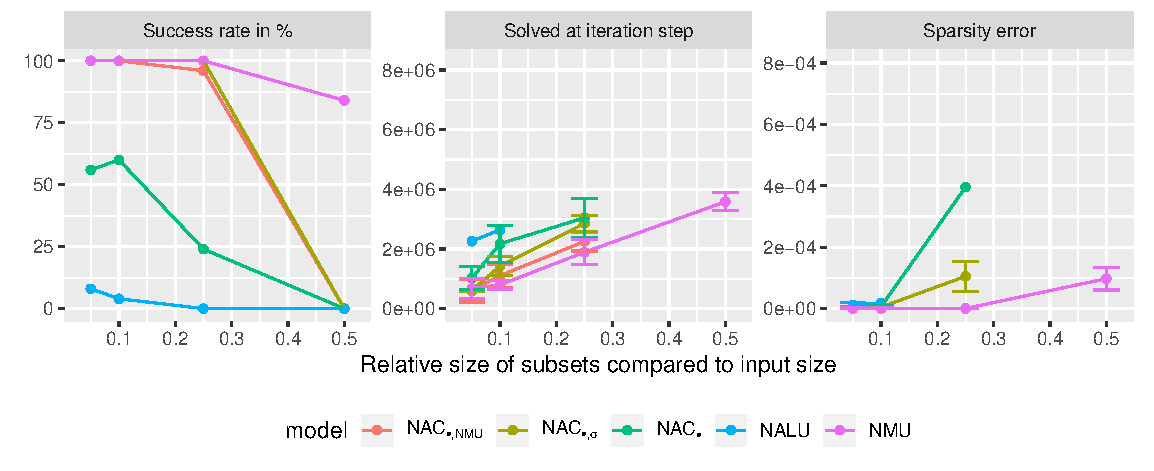
\includegraphics[width=\linewidth,trim={0 0 0 0.809cm},clip]{results/simple_function_static_mul_subset.pdf}
\caption{Shows the effect of the dataset parameters.}
\label{fig:simple-function-static-dataset-parameters-boundary}
\end{figure}

\subsection{Gating convergence experiment}
\label{sec:appendix:nalu-gate-experiment}

In the interest of adding some understand of what goes wrong in the NALU gate, and the shared weight choice that NALU employs to remedy this, we introduce the following experiment.

We train two models to fit the arithmetic task. Both uses the $\mathrm{NAC}_{+}$ in the first layer and NALU in the second layer. The only difference is that one model shares the weight between $\mathrm{NAC}_{+}$ and $\mathrm{NAC}_{\bullet}$ in the NALU, and the other treat them as two separate units with separate weights. In both cases NALU should gate between $\mathrm{NAC}_{+}$ and $\mathrm{NAC}_{\bullet}$ and choose the appropriate operation. Note that this NALU model is different from the one presented elsewhere in this paper, including the original NALU paper \cite{trask-nalu}. The typical NALU model is just two NALU layers with shared weights.

Furthermore, we also introduce a new gated unit that simply gates between our proposed NMU and NAU, using the same sigmoid gating-mechanism as in the NALU. This combination is done with seperate weights, as NMU and NAU use different weight constrains and can therefore not be shared.

The models are trained and evaluated over 100 different seeds on the multiplication and addition task. A histogram of the gate-value for all seeds is presented in figure \ref{fig:simple-function-static-nalu-gate-graph} and table \ref{tab:simple-function-static-nalu-gate-table} contains a summary. Some noteworthy observations:

\vspace{-0.3cm}\begin{enumerate}
    \item When the NALU weights are separated far more trials converge to select $\mathrm{NAC}_{+}$ for both the addition and multiplication task. Sharing the weights between $\mathrm{NAC}_{+}$ and $\mathrm{NAC}_{\bullet}$ makes the gating less likely to converge for addition.
    \item The performance of the addition task is dependent on NALU selecting the right operation. In the multiplication task, when the right gate is selected, $\mathrm{NAC}_{\bullet}$ do not converge consistently, unlike our NMU that converges more consistently.
    \item Which operation the gate converges to appears to be mostly random and independent of the task. These issues are caused by the sigmoid gating-mechanism and thus exists independent of the used sub-units.
\end{enumerate}

\vspace{-0.2cm}These observations validates that the NALU gating-mechanism does not converge as intended. This becomes a critical issues when more gates are present, as is normally the case. E.g. when stacking multiple NALU layers together.

\begin{figure}[h]
\centering
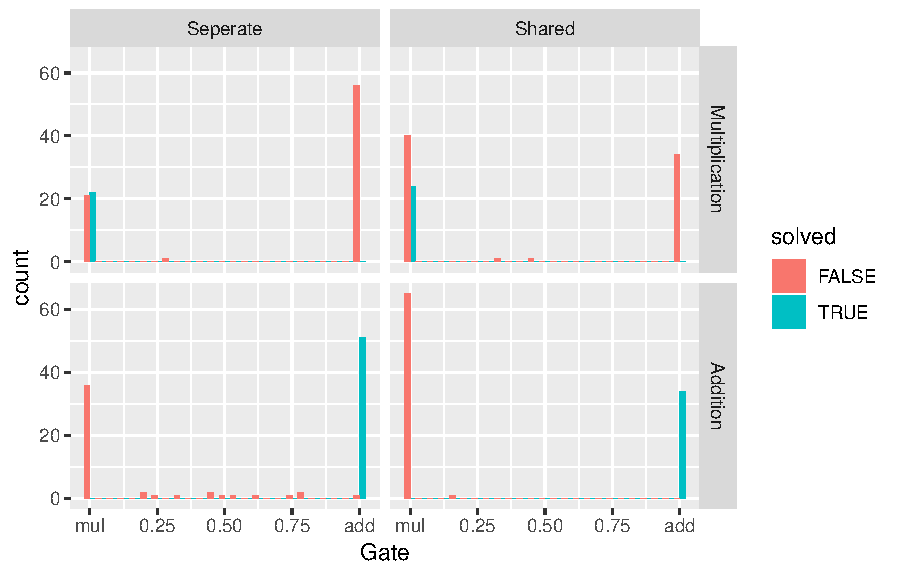
\includegraphics[width=0.93\linewidth]{results/function_task_static_nalu.pdf}
\vspace{-0.2cm}\caption{Shows the gating-value in the NALU layer and a variant that uses NAU/NMU instead of $\mathrm{NAC}_{+}$/$\mathrm{NAC}_{\bullet}$. Separate/shared refers to the weights in $\mathrm{NAC}_{+}$/$\mathrm{NAC}_{\bullet}$ used in NALU.}
\label{fig:simple-function-static-nalu-gate-graph}
\end{figure}

\begin{table}[!h]

\caption{\label{tab:simple-function-static-nalu-gate-table}Shows the success-rate, when the model converged, and the sparsity error for all weight matrices, with 95\% confidence interval. Each value is a summary of 100 different seeds.}
\centering
\begin{tabular}{crllll}
\toprule
\multicolumn{1}{c}{Op} & \multicolumn{1}{c}{Model} & \multicolumn{1}{c}{Success} & \multicolumn{2}{c}{Solved at} & \multicolumn{1}{c}{Sparsity error} \\
\cmidrule(l{3pt}r{3pt}){1-1} \cmidrule(l{3pt}r{3pt}){2-2} \cmidrule(l{3pt}r{3pt}){3-3} \cmidrule(l{3pt}r{3pt}){4-5} \cmidrule(l{3pt}r{3pt}){6-6}
 &  & Rate & Median & Mean & Mean\\
\midrule
 & Gated NAU/NMU & $\mathbf{62\%} {~}^{+9\%}_{-10\%}$ & $\mathbf{1.5 \cdot 10^{6}}$ & $\mathbf{1.5 \cdot 10^{6}} {~}^{+3.9 \cdot 10^{4}}_{-3.8 \cdot 10^{4}}$ & $\mathbf{5.0 \cdot 10^{-5}} {~}^{+2.3 \cdot 10^{-5}}_{-1.8 \cdot 10^{-5}}$\\

\nopagebreak
 & NALU (separate) & $22\% {~}^{+9\%}_{-7\%}$ & $2.8 \cdot 10^{6}$ & $3.3 \cdot 10^{6} {~}^{+3.9 \cdot 10^{5}}_{-3.6 \cdot 10^{5}}$ & $5.8 \cdot 10^{-2} {~}^{+4.1 \cdot 10^{-2}}_{-2.3 \cdot 10^{-2}}$\\

\nopagebreak
\multirow{-3}{*}{\centering\arraybackslash $\bm{\times}$} & NALU (shared) & $24\% {~}^{+9\%}_{-7\%}$ & $2.9 \cdot 10^{6}$ & $3.3 \cdot 10^{6} {~}^{+3.7 \cdot 10^{5}}_{-3.6 \cdot 10^{5}}$ & $1.0 \cdot 10^{-3} {~}^{+1.1 \cdot 10^{-3}}_{-4.5 \cdot 10^{-4}}$\\
\cmidrule{1-6}
 & Gated NAU/NMU & $37\% {~}^{+10\%}_{-9\%}$ & $\mathbf{1.9 \cdot 10^{4}}$ & $4.2 \cdot 10^{5} {~}^{+7.3 \cdot 10^{4}}_{-6.7 \cdot 10^{4}}$ & $\mathbf{1.7 \cdot 10^{-1}} {~}^{+4.6 \cdot 10^{-2}}_{-4.0 \cdot 10^{-2}}$\\

\nopagebreak
 & NALU (separate) & $\mathbf{51\%} {~}^{+10\%}_{-10\%}$ & $1.4 \cdot 10^{5}$ & $\mathbf{2.9 \cdot 10^{5}} {~}^{+3.5 \cdot 10^{4}}_{-4.3 \cdot 10^{4}}$ & $1.8 \cdot 10^{-1} {~}^{+1.4 \cdot 10^{-2}}_{-1.4 \cdot 10^{-2}}$\\

\nopagebreak
\multirow{-3}{*}{\centering\arraybackslash $\bm{+}$} & NALU (shared) & $34\% {~}^{+10\%}_{-9\%}$ & $1.8 \cdot 10^{5}$ & $3.1 \cdot 10^{5} {~}^{+4.3 \cdot 10^{4}}_{-5.4 \cdot 10^{4}}$ & $1.8 \cdot 10^{-1} {~}^{+2.3 \cdot 10^{-2}}_{-2.1 \cdot 10^{-2}}$\\
\bottomrule
\end{tabular}
\end{table}


\subsection{Regularization}
\label{sec:appendix:simple-function-task:regualization}

The $\lambda_{start}$ and $\lambda_{end}$ are simply selected based on how much time it takes for the model to converge. The sparsity regularizer should not be used during early optimization as this part of the optimization is exploratory and concerns finding the right solution by getting each weight on the right side of $\pm 0.5$.

In figure \ref{fig:simple-fnction-static-regularizer-add}, \ref{fig:simple-fnction-static-regularizer-sub} and \ref{fig:simple-fnction-static-regularizer-mul} the scaling factor $\hat{\lambda}_{\mathrm{sparse}}$ is optimized.
\begin{equation}
\lambda_{\mathrm{sparse}} = \hat{\lambda}_{\mathrm{sparse}} \max(\min(\frac{t - \lambda_{\mathrm{start}}}{\lambda_{\mathrm{end}} - \lambda_{\mathrm{start}}}, 1), 0)
\end{equation}

\begin{figure}[H]
\centering
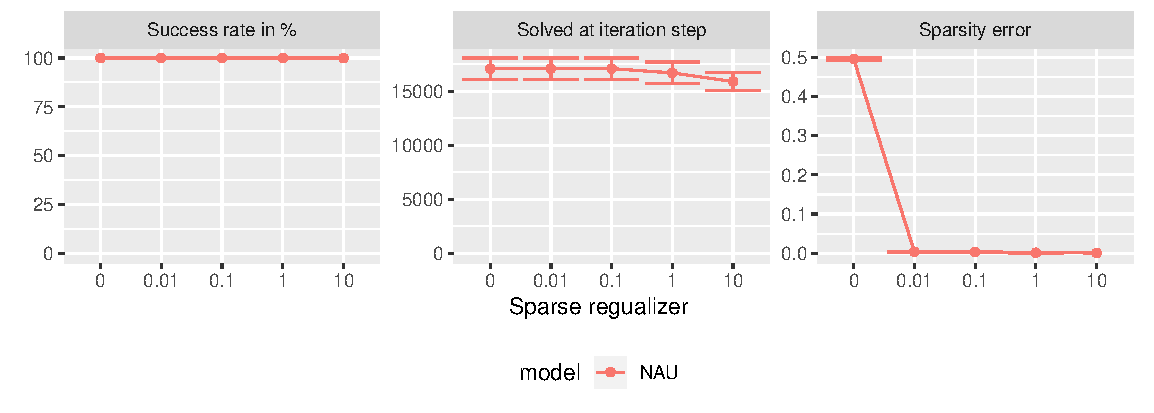
\includegraphics[width=\linewidth,trim={0 1.3cm 0 0},clip]{results/simple_function_static_regualization_add.pdf}
\caption{Shows effect of $\hat{\lambda}_{\mathrm{sparse}}$ in NAU on the arithmetic dataset for the $\bm{+}$ operation.}
\label{fig:simple-fnction-static-regularizer-add}
\end{figure}

\begin{figure}[H]
\centering
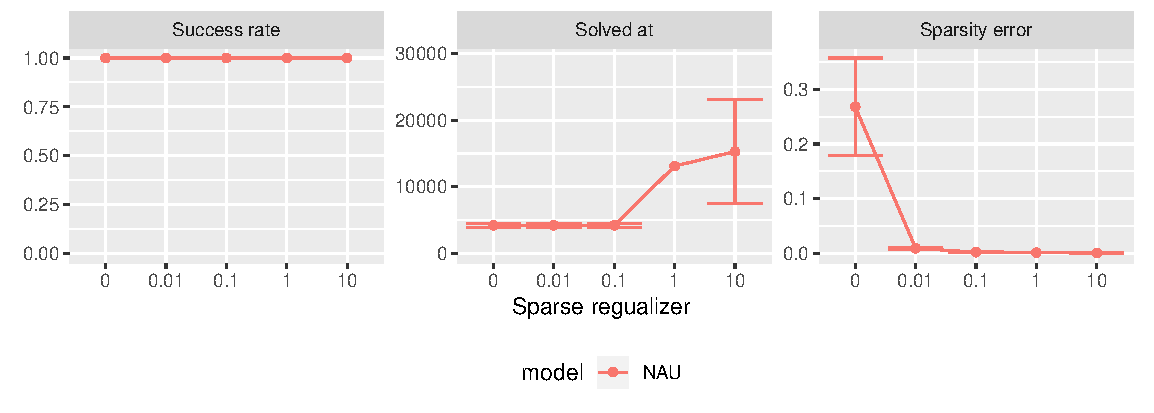
\includegraphics[width=\linewidth,trim={0 1.3cm 0 0},clip]{results/simple_function_static_regualization_sub.pdf}
\caption{Shows effect of $\hat{\lambda}_{\mathrm{sparse}}$ in NAU on the arithmetic dataset for the $\bm{-}$ operation.}
\label{fig:simple-fnction-static-regularizer-sub}
\end{figure}

\begin{figure}[H]
\centering
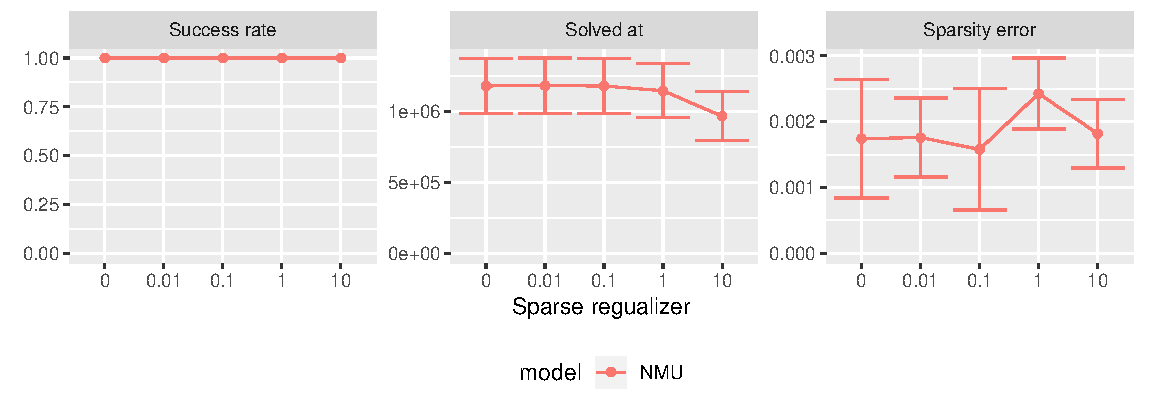
\includegraphics[width=\linewidth,trim={0 1.3cm 0 0},clip]{results/simple_function_static_regualization_mul.pdf}
\caption{Shows effect of $\hat{\lambda}_{\mathrm{sparse}}$ in NMU on the arithmetic dataset for the $\bm{\times}$ operation.}
\label{fig:simple-fnction-static-regularizer-mul}
\end{figure}

\subsection{Comparing all models}
\label{sec:appendix:comparison-all-models}

Table \ref{tab:function-task-static-defaults-all} compares all models on all operations used in NALU \cite{trask-nalu}. All variations of models and operations are trained for 100 different seeds to build confidence intervals. Some noteworthy observations are:

\begin{enumerate}
    \item Division does not work for any model, including the $\mathrm{NAC}_{\bullet}$ and NALU models. This may seem surprising but is actually in line with the results from the NALU paper (\citet{trask-nalu}, table 1) where there is a large error given the interpolation range. The extrapolation range has a smaller error, but this is an artifact of their evaluation method where they normalize with a random baseline. Since a random baseline will have a higher error for the extrapolation range, errors just appear to be smaller. A correct solution to division should have both a small interpolation and extrapolation error. 
    \item $\mathrm{NAC}_{\bullet}$ and NALU are barely able to learn $\sqrt{z}$, with just 2\% success-rate for NALU and 7\% success-rate for $\mathrm{NAC}_{\bullet}$.
    \item NMU is fully capable of learning $z^2$. It learn this by learning the same subset twice in the NAU layer, this is also how $\mathrm{NAC}_{\bullet}$ learn $z^2$.
    \item The Gated NAU/NMU (discussed in section \ref{sec:appendix:nalu-gate-experiment}) works very poorly, because the NMU initialization assumes that $E[z_{h_{\ell-1}}] = 0$. This is usually true, as discussed in section \ref{sec:methods:moments-and-initialization}, but not in this case for the first layer. In the recommended NMU model, the NMU layer appears after NAU, which causes that assumption to be satisfied.
\end{enumerate}


\begin{longtable}{crllll}
\caption{\label{tab:function-task-static-defaults-all}Shows the success-rate, when the model converged, and the sparsity error for all weight matrices, with 95\% confidence interval. Each value is a summary of 100 different seeds.}\\
\toprule
\multicolumn{1}{c}{Op} & \multicolumn{1}{c}{Model} & \multicolumn{1}{c}{Success} & \multicolumn{2}{c}{Solved at} & \multicolumn{1}{c}{Sparsity error} \\
\cmidrule(l{3pt}r{3pt}){1-1} \cmidrule(l{3pt}r{3pt}){2-2} \cmidrule(l{3pt}r{3pt}){3-3} \cmidrule(l{3pt}r{3pt}){4-5} \cmidrule(l{3pt}r{3pt}){6-6}
 &  & Rate & Median & Mean & Mean\\
\midrule
\endfirsthead
\caption[]{Shows the success-rate, when the model converged, and the sparsity error for all weight matrices, with 95\% confidence interval. Each value is a summary of 100 different seeds. \textit{(continued)}}\\
\toprule
\multicolumn{1}{c}{Op} & \multicolumn{1}{c}{Model} & \multicolumn{1}{c}{Success} & \multicolumn{2}{c}{Solved at} & \multicolumn{1}{c}{Sparsity error} \\
\cmidrule(l{3pt}r{3pt}){1-1} \cmidrule(l{3pt}r{3pt}){2-2} \cmidrule(l{3pt}r{3pt}){3-3} \cmidrule(l{3pt}r{3pt}){4-5} \cmidrule(l{3pt}r{3pt}){6-6}
 &  & Rate & Median & Mean & Mean\\
\midrule
\endhead
\
\endfoot
\bottomrule
\endlastfoot
 & $\mathrm{NAC}_{\bullet,\mathrm{NMU}}$ & $93\% {~}^{+4\%}_{-7\%}$ & $1.8 \cdot 10^{6}$ & $1.9 \cdot 10^{6} {~}^{+7.7 \cdot 10^{4}}_{-9.3 \cdot 10^{4}}$ & $9.5 \cdot 10^{-7} {~}^{+4.2 \cdot 10^{-7}}_{-4.2 \cdot 10^{-7}}$\\

\nopagebreak
 & $\mathrm{NAC}_{\bullet,\sigma}$ & $\mathbf{100\%} {~}^{+0\%}_{-4\%}$ & $2.5 \cdot 10^{6}$ & $2.6 \cdot 10^{6} {~}^{+8.8 \cdot 10^{4}}_{-7.2 \cdot 10^{4}}$ & $4.6 \cdot 10^{-5} {~}^{+5.0 \cdot 10^{-6}}_{-5.6 \cdot 10^{-6}}$\\

\nopagebreak
 & $\mathrm{NAC}_{\bullet}$ & $31\% {~}^{+10\%}_{-8\%}$ & $2.8 \cdot 10^{6}$ & $3.0 \cdot 10^{6} {~}^{+2.9 \cdot 10^{5}}_{-2.4 \cdot 10^{5}}$ & $5.8 \cdot 10^{-4} {~}^{+4.8 \cdot 10^{-4}}_{-2.6 \cdot 10^{-4}}$\\

\nopagebreak
 & $\mathrm{NAC}_{+}$ & $0\% {~}^{+4\%}_{-0\%}$ & --- & --- & ---\\

\nopagebreak
 & Linear & $0\% {~}^{+4\%}_{-0\%}$ & --- & --- & ---\\

\nopagebreak
 & NALU & $0\% {~}^{+4\%}_{-0\%}$ & --- & --- & ---\\

\nopagebreak
 & NAU & $0\% {~}^{+4\%}_{-0\%}$ & --- & --- & ---\\

\nopagebreak
 & NMU & $98\% {~}^{+1\%}_{-5\%}$ & $\mathbf{1.4 \cdot 10^{6}}$ & $\mathbf{1.5 \cdot 10^{6}} {~}^{+4.8 \cdot 10^{4}}_{-6.5 \cdot 10^{4}}$ & $\mathbf{4.2 \cdot 10^{-7}} {~}^{+2.9 \cdot 10^{-8}}_{-2.9 \cdot 10^{-8}}$\\

\nopagebreak
 & ReLU & $0\% {~}^{+4\%}_{-0\%}$ & --- & --- & ---\\

\nopagebreak
\multirow{-10}{*}{\centering\arraybackslash $\bm{\times}$} & ReLU6 & $0\% {~}^{+4\%}_{-0\%}$ & --- & --- & ---\\
\cmidrule{1-6}
 & $\mathrm{NAC}_{\bullet,\mathrm{NMU}}$ & $\mathbf{0\%} {~}^{+4\%}_{-0\%}$ & --- & --- & ---\\

\nopagebreak
 & $\mathrm{NAC}_{\bullet,\sigma}$ & $\mathbf{0\%} {~}^{+4\%}_{-0\%}$ & --- & --- & ---\\

\nopagebreak
 & $\mathrm{NAC}_{\bullet}$ & $\mathbf{0\%} {~}^{+4\%}_{-0\%}$ & --- & --- & ---\\

\nopagebreak
 & $\mathrm{NAC}_{+}$ & $\mathbf{0\%} {~}^{+4\%}_{-0\%}$ & --- & --- & ---\\

\nopagebreak
 & Linear & $\mathbf{0\%} {~}^{+4\%}_{-0\%}$ & --- & --- & ---\\

\nopagebreak
 & NALU & $\mathbf{0\%} {~}^{+4\%}_{-0\%}$ & --- & --- & ---\\

\nopagebreak
 & NAU & $\mathbf{0\%} {~}^{+4\%}_{-0\%}$ & --- & --- & ---\\

\nopagebreak
 & NMU & $\mathbf{0\%} {~}^{+4\%}_{-0\%}$ & --- & --- & ---\\

\nopagebreak
 & ReLU & $\mathbf{0\%} {~}^{+4\%}_{-0\%}$ & --- & --- & ---\\

\nopagebreak
\multirow{-10}{*}{\centering\arraybackslash $\bm{\mathbin{/}}$} & ReLU6 & $\mathbf{0\%} {~}^{+4\%}_{-0\%}$ & --- & --- & ---\\
\cmidrule{1-6}
 & $\mathrm{NAC}_{\bullet,\mathrm{NMU}}$ & $0\% {~}^{+4\%}_{-0\%}$ & --- & --- & ---\\

\nopagebreak
 & $\mathrm{NAC}_{\bullet,\sigma}$ & $0\% {~}^{+4\%}_{-0\%}$ & --- & --- & ---\\

\nopagebreak
 & $\mathrm{NAC}_{\bullet}$ & $0\% {~}^{+4\%}_{-0\%}$ & --- & --- & ---\\

\nopagebreak
 & $\mathrm{NAC}_{+}$ & $\mathbf{100\%} {~}^{+0\%}_{-4\%}$ & $2.5 \cdot 10^{5}$ & $4.9 \cdot 10^{5} {~}^{+5.2 \cdot 10^{4}}_{-4.5 \cdot 10^{4}}$ & $2.3 \cdot 10^{-1} {~}^{+6.5 \cdot 10^{-3}}_{-6.5 \cdot 10^{-3}}$\\

\nopagebreak
 & Linear & $\mathbf{100\%} {~}^{+0\%}_{-4\%}$ & $6.1 \cdot 10^{4}$ & $\mathbf{6.3 \cdot 10^{4}} {~}^{+2.5 \cdot 10^{3}}_{-3.3 \cdot 10^{3}}$ & $2.5 \cdot 10^{-1} {~}^{+3.6 \cdot 10^{-4}}_{-3.6 \cdot 10^{-4}}$\\

\nopagebreak
 & NALU & $14\% {~}^{+8\%}_{-5\%}$ & $1.5 \cdot 10^{6}$ & $1.6 \cdot 10^{6} {~}^{+3.8 \cdot 10^{5}}_{-3.3 \cdot 10^{5}}$ & $1.7 \cdot 10^{-1} {~}^{+2.7 \cdot 10^{-2}}_{-2.5 \cdot 10^{-2}}$\\

\nopagebreak
 & NAU & $\mathbf{100\%} {~}^{+0\%}_{-4\%}$ & $\mathbf{1.8 \cdot 10^{4}}$ & $3.9 \cdot 10^{5} {~}^{+4.4 \cdot 10^{4}}_{-3.7 \cdot 10^{4}}$ & $\mathbf{3.2 \cdot 10^{-5}} {~}^{+1.3 \cdot 10^{-5}}_{-1.3 \cdot 10^{-5}}$\\

\nopagebreak
 & NMU & $0\% {~}^{+4\%}_{-0\%}$ & --- & --- & ---\\

\nopagebreak
 & ReLU & $62\% {~}^{+9\%}_{-10\%}$ & $6.2 \cdot 10^{4}$ & $7.6 \cdot 10^{4} {~}^{+8.3 \cdot 10^{3}}_{-7.0 \cdot 10^{3}}$ & $2.5 \cdot 10^{-1} {~}^{+2.4 \cdot 10^{-3}}_{-2.4 \cdot 10^{-3}}$\\

\nopagebreak
\multirow{-10}{*}{\centering\arraybackslash $\bm{+}$} & ReLU6 & $0\% {~}^{+4\%}_{-0\%}$ & --- & --- & ---\\
\cmidrule{1-6}
 & $\mathrm{NAC}_{\bullet,\mathrm{NMU}}$ & $0\% {~}^{+4\%}_{-0\%}$ & --- & --- & ---\\

\nopagebreak
 & $\mathrm{NAC}_{\bullet,\sigma}$ & $0\% {~}^{+4\%}_{-0\%}$ & --- & --- & ---\\

\nopagebreak
 & $\mathrm{NAC}_{\bullet}$ & $0\% {~}^{+4\%}_{-0\%}$ & --- & --- & ---\\

\nopagebreak
 & $\mathrm{NAC}_{+}$ & $\mathbf{100\%} {~}^{+0\%}_{-4\%}$ & $9.0 \cdot 10^{3}$ & $3.7 \cdot 10^{5} {~}^{+3.8 \cdot 10^{4}}_{-3.8 \cdot 10^{4}}$ & $2.3 \cdot 10^{-1} {~}^{+5.4 \cdot 10^{-3}}_{-5.4 \cdot 10^{-3}}$\\

\nopagebreak
 & Linear & $7\% {~}^{+7\%}_{-4\%}$ & $3.3 \cdot 10^{6}$ & $1.4 \cdot 10^{6} {~}^{+7.0 \cdot 10^{5}}_{-6.1 \cdot 10^{5}}$ & $1.8 \cdot 10^{-1} {~}^{+7.2 \cdot 10^{-2}}_{-5.8 \cdot 10^{-2}}$\\

\nopagebreak
 & NALU & $14\% {~}^{+8\%}_{-5\%}$ & $1.9 \cdot 10^{6}$ & $1.9 \cdot 10^{6} {~}^{+4.4 \cdot 10^{5}}_{-4.5 \cdot 10^{5}}$ & $2.1 \cdot 10^{-1} {~}^{+2.2 \cdot 10^{-2}}_{-2.2 \cdot 10^{-2}}$\\

\nopagebreak
 & NAU & $\mathbf{100\%} {~}^{+0\%}_{-4\%}$ & $\mathbf{5.0 \cdot 10^{3}}$ & $\mathbf{1.6 \cdot 10^{5}} {~}^{+1.7 \cdot 10^{4}}_{-1.6 \cdot 10^{4}}$ & $6.6 \cdot 10^{-2} {~}^{+2.5 \cdot 10^{-2}}_{-1.9 \cdot 10^{-2}}$\\

\nopagebreak
 & NMU & $56\% {~}^{+9\%}_{-10\%}$ & $1.0 \cdot 10^{6}$ & $1.0 \cdot 10^{6} {~}^{+5.8 \cdot 10^{2}}_{-5.8 \cdot 10^{2}}$ & $\mathbf{3.4 \cdot 10^{-4}} {~}^{+3.2 \cdot 10^{-5}}_{-2.6 \cdot 10^{-5}}$\\

\nopagebreak
 & ReLU & $0\% {~}^{+4\%}_{-0\%}$ & --- & --- & ---\\

\nopagebreak
\multirow{-10}{*}{\centering\arraybackslash $\bm{-}$} & ReLU6 & $0\% {~}^{+4\%}_{-0\%}$ & --- & --- & ---\\
\cmidrule{1-6}
 & $\mathrm{NAC}_{\bullet,\mathrm{NMU}}$ & $3\% {~}^{+5\%}_{-2\%}$ & $1.0 \cdot 10^{6}$ & $\mathbf{1.0 \cdot 10^{6}}$ & $\mathbf{1.7 \cdot 10^{-1}} {~}^{+8.3 \cdot 10^{-3}}_{-8.1 \cdot 10^{-3}}$\\

\nopagebreak
 & $\mathrm{NAC}_{\bullet,\sigma}$ & $0\% {~}^{+4\%}_{-0\%}$ & --- & --- & ---\\

\nopagebreak
 & $\mathrm{NAC}_{\bullet}$ & $\mathbf{7\%} {~}^{+7\%}_{-4\%}$ & $\mathbf{4.0 \cdot 10^{5}}$ & $1.5 \cdot 10^{6} {~}^{+6.0 \cdot 10^{5}}_{-5.6 \cdot 10^{5}}$ & $2.4 \cdot 10^{-1} {~}^{+1.7 \cdot 10^{-2}}_{-1.7 \cdot 10^{-2}}$\\

\nopagebreak
 & $\mathrm{NAC}_{+}$ & $0\% {~}^{+4\%}_{-0\%}$ & --- & --- & ---\\

\nopagebreak
 & Linear & $0\% {~}^{+4\%}_{-0\%}$ & --- & --- & ---\\

\nopagebreak
 & NALU & $2\% {~}^{+5\%}_{-1\%}$ & $2.6 \cdot 10^{6}$ & $3.3 \cdot 10^{6} {~}^{+1.8 \cdot 10^{6}}_{-2.2 \cdot 10^{6}}$ & $5.0 \cdot 10^{-1} {~}^{+2.5 \cdot 10^{-6}}_{-8.0 \cdot 10^{-6}}$\\

\nopagebreak
 & NAU & $0\% {~}^{+4\%}_{-0\%}$ & --- & --- & ---\\

\nopagebreak
 & NMU & $0\% {~}^{+4\%}_{-0\%}$ & --- & --- & ---\\

\nopagebreak
 & ReLU & $0\% {~}^{+4\%}_{-0\%}$ & --- & --- & ---\\

\nopagebreak
\multirow{-10}{*}{\centering\arraybackslash $\sqrt{z}$} & ReLU6 & $0\% {~}^{+4\%}_{-0\%}$ & --- & --- & ---\\
\cmidrule{1-6}
 & $\mathrm{NAC}_{\bullet,\mathrm{NMU}}$ & $\mathbf{100\%} {~}^{+0\%}_{-4\%}$ & $1.4 \cdot 10^{6}$ & $1.5 \cdot 10^{6} {~}^{+7.1 \cdot 10^{4}}_{-5.9 \cdot 10^{4}}$ & $\mathbf{2.9 \cdot 10^{-7}} {~}^{+1.4 \cdot 10^{-8}}_{-1.4 \cdot 10^{-8}}$\\

\nopagebreak
 & $\mathrm{NAC}_{\bullet,\sigma}$ & $\mathbf{100\%} {~}^{+0\%}_{-4\%}$ & $1.9 \cdot 10^{6}$ & $1.9 \cdot 10^{6} {~}^{+5.3 \cdot 10^{4}}_{-6.2 \cdot 10^{4}}$ & $1.8 \cdot 10^{-2} {~}^{+4.3 \cdot 10^{-4}}_{-4.3 \cdot 10^{-4}}$\\

\nopagebreak
 & $\mathrm{NAC}_{\bullet}$ & $77\% {~}^{+7\%}_{-9\%}$ & $3.3 \cdot 10^{6}$ & $3.2 \cdot 10^{6} {~}^{+1.6 \cdot 10^{5}}_{-2.0 \cdot 10^{5}}$ & $1.8 \cdot 10^{-2} {~}^{+5.8 \cdot 10^{-4}}_{-5.7 \cdot 10^{-4}}$\\

\nopagebreak
 & $\mathrm{NAC}_{+}$ & $0\% {~}^{+4\%}_{-0\%}$ & --- & --- & ---\\

\nopagebreak
 & Linear & $0\% {~}^{+4\%}_{-0\%}$ & --- & --- & ---\\

\nopagebreak
 & NALU & $0\% {~}^{+4\%}_{-0\%}$ & --- & --- & ---\\

\nopagebreak
 & NAU & $0\% {~}^{+4\%}_{-0\%}$ & --- & --- & ---\\

\nopagebreak
 & NMU & $\mathbf{100\%} {~}^{+0\%}_{-4\%}$ & $\mathbf{1.2 \cdot 10^{6}}$ & $\mathbf{1.3 \cdot 10^{6}} {~}^{+3.1 \cdot 10^{4}}_{-3.6 \cdot 10^{4}}$ & $3.7 \cdot 10^{-5} {~}^{+5.4 \cdot 10^{-5}}_{-3.7 \cdot 10^{-5}}$\\

\nopagebreak
 & ReLU & $0\% {~}^{+4\%}_{-0\%}$ & --- & --- & ---\\

\nopagebreak
\multirow{-10}{*}{\centering\arraybackslash $z^2$} & ReLU6 & $0\% {~}^{+4\%}_{-0\%}$ & --- & --- & ---\\*
\end{longtable}
